\documentclass[11pt,a4paper]{article}

% ---------------------------------------------------------------------------
% Complex-balanced realizations of a coupled autocatalytic assembly:
% exact obstructions, an explicit disguised-toric locus, and global dynamics.
%
% Author metadata: set the three macros below before submission.
% ---------------------------------------------------------------------------
\newcommand{\PaperAuthor}{}
\newcommand{\PaperAffiliation}{}
\newcommand{\PaperDate}{September 2026}

\usepackage[T1]{fontenc}
\usepackage[utf8]{inputenc}
\usepackage{lmodern}
\usepackage{microtype}
\usepackage[a4paper,margin=1.05in]{geometry}
\usepackage{amsmath,amssymb,amsthm,mathtools}
\usepackage{booktabs}
\usepackage{array}
\usepackage{enumitem}
\usepackage{graphicx}
\usepackage{xcolor}
\usepackage[obeyspaces,spaces]{url}
\usepackage[colorlinks=true,linkcolor=blue!55!black,citecolor=blue!55!black,urlcolor=blue!55!black]{hyperref}

\setlist{itemsep=2pt,topsep=3pt}
\setlength{\emergencystretch}{1.5em}

\theoremstyle{plain}
\newtheorem{theorem}{Theorem}[section]
\newtheorem{proposition}[theorem]{Proposition}
\newtheorem{lemma}[theorem]{Lemma}
\newtheorem{corollary}[theorem]{Corollary}
\theoremstyle{definition}
\newtheorem{definition}[theorem]{Definition}
\newtheorem{example}[theorem]{Example}
\newtheorem{question}[theorem]{Question}
\theoremstyle{remark}
\newtheorem{remark}[theorem]{Remark}

\newcommand{\R}{\mathbb{R}}
\newcommand{\N}{\mathbb{N}}
\newcommand{\Rp}{\R_{>0}}
\newcommand{\DT}{\mathcal{D}}
\newcommand{\cc}{\mathsf{c}}
\newcommand{\rA}{\mathcal{A}}
\newcommand{\rB}{\mathcal{B}}
\newcommand{\rK}{\mathcal{K}}
\newcommand{\rH}{\mathcal{H}}
\newcommand{\xs}{x^{*}}
\newcommand{\diag}{\operatorname{diag}}
\newcommand{\rev}[2]{\mathrel{\mathop{\rightleftarrows}\limits^{#1}_{#2}}}
\DeclareUrlCommand\lean{\urlstyle{tt}}

\title{Complex-balanced realizations of a coupled autocatalytic assembly:\\ exact obstructions, an explicit disguised-toric locus,\\ and global dynamics}
\author{\PaperAuthor\\ \PaperAffiliation}
\date{\PaperDate}

\begin{document}
\maketitle

\begin{abstract}
A mass-action system is disguised toric if some other mass-action network on the same species has the same polynomial vector field and is complex balanced; complex balance then supplies a unique, globally attracting positive equilibrium through the Horn--Jackson entropy. We compute the disguised-toric locus exactly for a literal six-parameter family of four-species mass-action systems that arises as a driven assembly of two minimal autocatalytic cores. At a positive stationary state, two explicit flux budgets, $K=A-Bz\ge0$ and $J=e(B-A^2)\le B$, are necessary and sufficient for the existence of a dynamically equivalent complex-balanced realization, even when the competing realization may use any finite set of auxiliary complexes of any molecularity. Necessity is proved by two supporting-plane certificates, each a piecewise-affine convex function on exponent space whose supporting inequalities are checked at all $64$ ordered pairs of source complexes and extended to arbitrary auxiliary vertices; sufficiency is proved by an explicit nineteen-edge balanced flux table whose rate constants reconstruct the entire polynomial field. A one-variable monotone elimination removes the stationary state and yields a quantifier-free criterion in the six rate constants, with both equality boundaries included. The state and parameter criteria, the rate reconstruction, and the full vector-field equality are kernel-checked in Lean~4 with Mathlib. We then prove permanence of every positive trajectory for all positive parameters and global asymptotic stability of the balancing state on the whole locus. An exact rational slice crosses the boundary of the locus while its unique equilibrium stays hyperbolic, locally stable, and productive for one core, and a uniform Lyapunov estimate transfers global stability to an open set of nontoric parameters. Finally, the classification is invariant under adjoining any finite number of reversible catalytic attachments of private species.
\end{abstract}

\noindent\textbf{Keywords.} chemical reaction networks; mass-action kinetics; complex balance; disguised toric locus; dynamical equivalence; autocatalytic cores; global stability; formal verification.

\medskip
\noindent\textbf{MSC 2020.} 80A30, 92C42, 37N25, 34D23, 52A20, 68V20.

\section{Introduction}\label{sec:intro}

Complex-balanced mass-action systems form the best understood class of polynomial dynamical systems arising in chemistry. Horn and Jackson showed that complex balance at one positive state forces a unique positive equilibrium in every stoichiometric compatibility class, together with a strict entropy-like Lyapunov function~\cite{HornJackson1972}; Horn and Feinberg characterized the rate constants at which a fixed network is complex balanced by a polynomial variety of codimension equal to the deficiency~\cite{Horn1972,Feinberg1972,Feinberg2019}, the \emph{toric locus} in the language of~\cite{CDSS2009}. Because the vector field is the only observable of a mass-action model, the same polynomial field is typically generated by many different networks and rate constants~\cite{CraciunPantea2008,Szederkenyi2010,JohnstonSiegel2011}. A system is called \emph{disguised toric} if some dynamically equivalent network is complex balanced~\cite{BrustengaCraciunSorea2022}; it then inherits every consequence of complex balance although its own graph need not be weakly reversible and its own rate constants need not satisfy any toric constraint. The \emph{disguised toric locus} of a network is the set of rate constants with this property. It is invariant under affine equivalence of networks~\cite{HaqueSatrianoSoreaYu2023}, path connected~\cite{CraciunDeshpandeJin2024}, and, in the recent flux-based analysis of Boros, Craciun, Henriksson, Jin and Rojas La Luz, a contractible manifold with boundary admitting a graph-theoretic description~\cite{Boros2026}; M\"uller, Deshpande and Regensburger reformulate the membership problem in the language of positive algebraic geometry~\cite{MullerDeshpandeRegensburger2026}. Exact, closed-form descriptions of the locus for specific networks of modelling interest remain rare, because membership couples a linear flux problem at a fixed state with the nonlinear problem of finding a common balancing state.

This paper computes the disguised-toric locus exactly for a family of four-species systems that arises in the theory of autocatalytic reaction networks. Following Blokhuis, Lacoste and Nghe~\cite{BlokhuisLacosteNghe2020}, a minimal autocatalytic core is a smallest subnetwork whose stoichiometry admits a strictly positive net production of all its members; Nandan, Nghe and Unterberger~\cite{NandanNgheUnterberger2026} classify such cores and study their coupling, extending a three-species multistationary example of Joshi, Kaihnsa, Nguyen and Shiu~\cite{JoshiKaihnsaNguyenShiu2023}. The companion manuscript~\cite{FeedbackBistability2026} studies the driven assembly of two gain-two cores
\begin{equation}\label{eq:source}
\begin{gathered}
A\rev{1}{1}B+z,\qquad z\rev{u}{1}H,\qquad 2z\rev{v}{1}H,\\
0\rev{a}{1}A,\qquad 0\rev{b}{1}B,\qquad B\rev{e}{e}2A,\qquad H\xrightarrow{\ d\ }0,
\end{gathered}
\end{equation}
with parameters $p=(a,b,u,v,e,d)\in\Rp^6$, upper labels for the left-to-right reactions, and $0$ denoting exchange with reservoirs held at unit activity. Its mass-action equations are
\begin{equation}\label{eq:ode}
\begin{aligned}
\dot A&=a-2A+Bz+2e(B-A^2),\\
\dot B&=b+A-(1+z)B-e(B-A^2),\\
\dot z&=A-Bz-uz-2vz^2+3H,\\
\dot H&=uz+vz^2-(2+d)H,
\end{aligned}
\end{equation}
and we write $f_p:\R^4\to\R^4$ for the right-hand side. The $AB$ core is formed by the fork $A\rightleftarrows B+z$ and the reverse channel $B\rightleftarrows2A$ restricted to $(A,B)$; the $zH$ core by $z\rightleftarrows H$ and $H\rightleftarrows2z$ restricted to $(z,H)$. The tied rate constants and the irreversible output are part of the model, so the six free parameters trace a six-dimensional section of the thirteen-dimensional rate space of the network~\eqref{eq:source}. The companion manuscript proves that the assembly has exactly one positive equilibrium whenever $d\ge1$, and exhibits bistability in an explicit parameter family with small reverse-channel rate $e$. Here we ask for which parameters the assembly is secretly complex balanced, and what this implies for its trajectories.

\subsection{Main results}\label{sec:main}

Throughout, a \emph{realization} of $f_p$ is a finite mass-action system on the species $A,B,z,H$, with complexes in $\N^4$ and nonnegative rate constants, whose polynomial vector field equals $f_p$ identically. No bound on the number or molecularity of its complexes is imposed. At a positive state $x=(A,B,z,H)$ put
\begin{equation}\label{eq:KJ}
K=A-Bz,\qquad J=e(B-A^2),
\end{equation}
the net currents of the fork and of the reverse channel.

\begin{theorem}[State criterion; Theorem~\ref{thm:state}]\label{thm:A}
Let $p\in\Rp^6$ and $x\in\Rp^4$. A realization of $f_p$ that is complex balanced at $x$ exists if and only if
\[
f_p(x)=0,\qquad K\ge0,\qquad J\le B.
\]
When these hold, a realization exists whose complexes are exactly the eight source complexes of~\eqref{eq:source}, with the explicit rate constants of Table~\ref{tab:flux}.
\end{theorem}

To eliminate the state, let $c=a+2b$, $s=a+b$, and define on $z>-2$
\begin{equation}\label{eq:reduced}
\begin{gathered}
\rB(z)=\frac{c}{z+2},\qquad
\rK(z)=\frac{v(1+2d)z^2-u(1-d)z}{2+d},\qquad
\rA(z)=z\rB(z)+\rK(z),\\
E(z)=b-(1+e)\rB(z)+\rK(z)+e\rA(z)^2,
\end{gathered}
\end{equation}
together with the two cut points
\begin{equation}\label{eq:cuts}
z_0=\max\Bigl\{0,\frac{u(1-d)}{v(1+2d)}\Bigr\},\qquad
t=\frac{c(e-1)}{es^2}-2.
\end{equation}

\begin{theorem}[Parameter locus; Theorem~\ref{thm:locus}]\label{thm:B}
The disguised-toric locus $\DT\subset\Rp^6$ of the family~\eqref{eq:ode} consists exactly of the parameters with
\[
E(z_0)\le0\quad\text{and}\quad\bigl[\,e\le1\ \ \text{or}\ \ t\le z_0\ \ \text{or}\ \ \rA(t)\le s\,\bigr].
\]
For $p\in\DT$ the function $E$ has a unique root $z_*$ on $[z_0,\infty)$, it is positive, and $\xs=(\rA(z_*),\rB(z_*),z_*,\rH(z_*))$ with $\rH(z)=(uz+vz^2)/(2+d)$ is the balancing state of Theorem~\ref{thm:A}. In particular $\{d\ge1,\ e\le1\}\subset\DT$.
\end{theorem}

The third alternative is only evaluated when $t>z_0\ge0$, so that $\rB(t)$ is defined; both equality boundaries $E(z_0)=0$ and $\rA(t)=s$ belong to $\DT$. The quantities in Theorems~\ref{thm:A} and~\ref{thm:B}, the reconstruction of the rate constants, and the identity of the whole polynomial field are verified in Lean~4~\cite{Lean4,Mathlib}; Appendix~\ref{app:formal} records the statements and the verification receipts.

\begin{theorem}[Permanence and global stability; Theorems~\ref{thm:permanence} and~\ref{thm:gas}]\label{thm:C}
For every $p\in\Rp^6$, every positive initial state has a unique global positive solution of~\eqref{eq:ode}, and there are constants $0<m<M$, depending only on $p$ and uniform on compact parameter sets, such that every such solution eventually remains in $[m,M]^4$. For every $p\in\DT$ the balancing state $\xs$ is the unique positive equilibrium and is globally asymptotically stable relative to $\Rp^4$.
\end{theorem}

\begin{theorem}[A stable productive crossing; Proposition~\ref{prop:slice} and Theorem~\ref{thm:open}]\label{thm:D}
On the rational slice $p_\eta=\bigl(\tfrac{19-2\eta}{25},\tfrac{\eta-4}{25},1,5,\eta,3\bigr)$, $4<\eta<\tfrac{19}{2}$, the point $\xs=(\tfrac25,\tfrac15,\tfrac15,\tfrac2{25})$ is the unique positive equilibrium, hyperbolic and locally asymptotically stable for every $\eta$, disguised toric exactly when $\eta\le5$, and strictly productive for the $AB$ core exactly when $\tfrac92<\eta<9$. There is a nonempty open subset of $\Rp^6\setminus\DT$ on which every system has a unique, globally asymptotically stable positive equilibrium with a strictly productive $AB$ core.
\end{theorem}

\begin{theorem}[Catalytic attachments; Theorem~\ref{thm:assembly}]\label{thm:E}
Adjoin to~\eqref{eq:source} any finite family of reversible reactions $Y_r\rightleftarrows Y_r+W_r$ with private species $W_r$, arbitrary catalyst complexes $Y_r\in\N^4$ in the base species, and positive rate constants. The enlarged system is disguised toric if and only if $p\in\DT$, with the same criterion as Theorem~\ref{thm:B}, even against competing realizations that use arbitrary mixed complexes in the enlarged species space. Permanence and global asymptotic stability transfer from the base system.
\end{theorem}

\subsection{Methods}\label{sec:methods}

The necessity half of Theorem~\ref{thm:A} is the technical heart of the paper. A complex-balanced realization at $x$ is a nonnegative flux on a finite directed graph whose vertex set contains the eight source complexes, with vertex balance at every vertex and prescribed \emph{coefficient drift} $\sum_j q_{ij}(y_j-y_i)$ at every vertex: the coefficient vector of the monomial $x^{y_i}$ in $f_p$ at source complexes and zero at every auxiliary complex. Suppose vectors $h_i$ and scalars $\pi_i$ satisfy $h_i\cdot(y_j-y_i)+\pi_j-\pi_i\ge0$ for all ordered pairs of vertices. Multiplying by $q_{ij}$ and summing, vertex balance cancels the potentials and what remains is $\sum_ih_i\cdot(\text{drift}_i)\ge0$, a linear inequality in the coefficient rows. The point is that such supporting data at the eight source complexes extend to \emph{any} finite set of auxiliary vertices: the pieces $\pi_i-h_i\cdot(y-y_i)$ define a convex piecewise-affine function $F$ on exponent space, and choosing at each auxiliary vertex an active piece supplies compatible data there. Auxiliary vertices have zero drift, so they contribute nothing to the pairing. Two such certificates, given in Table~\ref{tab:dual}, pair the coefficient rows of~\eqref{eq:ode} to $K$ and to $2(B-J)$; the first comes from $F_K(y)=-\min(y_B,y_z)$ and needs no stationarity, the second uses $\dot H=0$ and $\dot A+\dot B=0$. This certificate argument proves both obstructions against all finite auxiliary complexes at once, without invoking source-reduction theorems for realizations~\cite{CraciunJinYu2020}. Sufficiency is a nineteen-entry flux table on the source complexes, balanced at every vertex by the stationarity identities; dividing by source monomials gives rate constants whose network has exactly the field $f_p$.

The parameter criterion follows a one-variable elimination. Adding $\dot A$ to $2\dot B$ gives $B=\rB(z)$ at stationarity, and $(2+d)\dot z+3\dot H=0$ gives $K=\rK(z)$; the remaining equation is $E(z)=0$. The current $K$ is nonnegative exactly on $z\ge z_0$, where $\rK$, $\rA$ and $E$ are increasing, so an admissible root exists if and only if $E(z_0)\le0$. The reservoir bound $J\le B$ is the inequality $\rA(z_*)\le s$, and an exact factorization, $(\rA-s)(1+e(\rA+s))=(e-1)\rB-es^2$ at the root, converts it into the comparison $t\le z_*$, which the monotone function $E$ evaluates directly at $t$ as $E(t)=(\rA(t)-s)(1+e(\rA(t)+s))$.

The dynamical results use the entropy $G(x\mid\xs)=\sum_k(x_k\log(x_k/x_k^*)-x_k+x_k^*)$ of a complex-balanced realization together with a permanence theorem proved directly from the literal feeds and outputs, avoiding any general persistence conjecture; the stoichiometric subspace is all of $\R^4$ by a determinant $-(a+b)uv$ of four coefficient rows, so equality in the entropy inequality forces $x=\xs$. The stable crossing uses the exact characteristic polynomial of a rational slice and the Routh--Hurwitz criterion, and the open nontoric region uses a uniform quadratic Lyapunov decrease near a moving equilibrium branch on a common absorbing box.

\subsection{Formal and conventional evidence}\label{sec:evidence}

The Lean development covers Theorems~\ref{thm:A} and~\ref{thm:B} completely, including the unrestricted quantifier over auxiliary complexes, the explicit rate constants, the identity of the whole polynomial vector field, the safe region, the rational examples, the algebraic identities behind permanence, and the algebra of the rational slice (stationarity, uniqueness, toric threshold, productivity interval, and the sign of all Hurwitz quantities for every $\eta>0$). The trajectory statements of Theorem~\ref{thm:C}, the Routh--Hurwitz and linearization steps of Theorem~\ref{thm:D}, the perturbation argument, and Theorem~\ref{thm:E} are conventional proofs given in full below and are not claimed to be formalized. Appendix~\ref{app:formal} lists the division claim by claim. A small script re-verifies every number printed in this paper in exact rational arithmetic.

\subsection{Organization}

Section~\ref{sec:prelim} fixes definitions and records the coefficient rows and the reduced functions. Section~\ref{sec:dual} proves the certificate lemmas and the necessity of the two flux budgets; Section~\ref{sec:flux} gives the realizing flux table and completes the proof of Theorem~\ref{thm:A}. Section~\ref{sec:locus} proves Theorem~\ref{thm:B} and gives exact examples. Section~\ref{sec:dynamics} proves permanence and global stability, Section~\ref{sec:crossing} the stable crossing and the open nontoric region, and Section~\ref{sec:assembly} the catalytic attachment theorem. Section~\ref{sec:discussion} discusses scope and open questions. Appendix~\ref{app:formal} describes the formal development and reproduction.

\section{Preliminaries}\label{sec:prelim}

\subsection{Mass-action systems, realizations and complex balance}

Let $n$ be the number of species. For $y\in\N^n$ and $x\in\Rp^n$ write $x^y=\prod_kx_k^{y_k}$. A \emph{mass-action system} is a finite set $\mathcal Y\subset\N^n$ of complexes together with rate constants $k_{ij}\ge0$ for ordered pairs of distinct complexes; its vector field is
\begin{equation}\label{eq:field}
f(x)=\sum_{i,j}k_{ij}\,x^{y_i}\,(y_j-y_i),
\end{equation}
and the reactions of the system are the pairs with $k_{ij}>0$. Two systems on the same species are \emph{dynamically equivalent} if their vector fields agree as polynomial maps; a system dynamically equivalent to a given one is a \emph{realization} of it. The system is \emph{complex balanced at $\xs\in\Rp^n$} if
\begin{equation}\label{eq:balance}
\sum_jk_{ij}(\xs)^{y_i}=\sum_jk_{ji}(\xs)^{y_j}\qquad\text{for every complex }y_i,
\end{equation}
that is, if the flux $q_{ij}=k_{ij}(\xs)^{y_i}$ is a circulation on the reaction graph. Summing~\eqref{eq:balance} against $y_i$ shows $f(\xs)=0$. A system is \emph{disguised toric} if it has a realization that is complex balanced at some positive state~\cite{BrustengaCraciunSorea2022}; the disguised-toric locus of a network is the set of its rate constants with this property. For the family~\eqref{eq:ode} we write
\[
\DT=\{p\in\Rp^6:\ f_p\ \text{has a complex-balanced realization}\},
\]
the pullback of the disguised-toric locus of the network~\eqref{eq:source} under the tied parameterization.

Write a polynomial vector field with finitely many monomials as $f(x)=\sum_ix^{y_i}\cc_i$ with distinct exponents $y_i$ and nonzero coefficient vectors $\cc_i\in\R^n$; the $y_i$ are the \emph{source complexes} of $f$. Distinct monomials are linearly independent as functions on $\Rp^n$, so a realization~\eqref{eq:field} of $f$ must contain every source complex of $f$, and coefficient matching reads
\begin{equation}\label{eq:drift}
\sum_jk_{ij}(y_j-y_i)=\cc_i\ \text{at source complexes},\qquad
\sum_jk_{ij}(y_j-y_i)=0\ \text{at every other complex}.
\end{equation}
Multiplying~\eqref{eq:drift} by $(\xs)^{y_i}$ expresses it in terms of fluxes. We call $r_i=(\xs)^{y_i}\cc_i$ the \emph{coefficient row} of the source complex $y_i$ at $\xs$ and $\sum_jq_{ij}(y_j-y_i)$ the \emph{coefficient drift} of vertex $i$. In summary: a complex-balanced realization at $\xs$ is a nonnegative flux $q$ on a finite vertex set containing the source complexes, with zero diagonal, vertex balance~\eqref{eq:balance} at every vertex, drift $r_i$ at source complexes and drift zero elsewhere. This is the representation used in the formal development (Appendix~\ref{app:formal}).

\subsection{The assembly and its coefficient rows}

Order the source complexes of~\eqref{eq:ode} as
\[
(0,\ A,\ B+z,\ z,\ H,\ 2z,\ B,\ 2A),
\]
with coordinates ordered $(A,B,z,H)$. The coefficient vectors $\cc_i$ are read off from~\eqref{eq:ode}:
\begin{equation}\label{eq:rows}
\begin{array}{c|rrrr}
y_i&\cc_{i,A}&\cc_{i,B}&\cc_{i,z}&\cc_{i,H}\\\hline
0&a&b&0&0\\
A&-2&1&1&0\\
B+z&1&-1&-1&0\\
z&0&0&-u&u\\
H&0&0&3&-(2+d)\\
2z&0&0&-2v&v\\
B&2e&-(1+e)&0&0\\
2A&-2e&e&0&0
\end{array}
\end{equation}
The rows $z$, $H$ and $2z$ record that $H\to z$ and $H\to2z$ together contribute $3H$ to $\dot z$. At a positive state the coefficient row is $r_i=x^{y_i}\cc_i$, with source monomials $1,A,Bz,z,H,z^2,B,A^2$.

\subsection{Stationary reconstruction}

Two exact combinations of~\eqref{eq:ode} expose the stationary set:
\begin{equation}\label{eq:combinations}
\dot A+2\dot B=c-(z+2)B,\qquad
(2+d)\dot z+3\dot H=(2+d)(A-Bz)-u(d-1)z-v(1+2d)z^2.
\end{equation}
Hence at a stationary state $B=\rB(z)$, $K=\rK(z)$, $A=\rA(z)$, $H=\rH(z)$ with the functions of~\eqref{eq:reduced}, and the remaining equation $\dot B=0$ becomes $E(z)=0$. Conversely, for the \emph{lift} $\ell(z)=(\rA(z),\rB(z),z,\rH(z))$ one has $\dot z=\dot H=0$, $\dot B=E(z)$ and $\dot A=-2E(z)$, so $\ell(z)$ is stationary exactly when $E(z)=0$. Positive stationary states therefore correspond bijectively to roots $z>0$ of $E$ with $\rA(z)>0$; the last condition is automatic on $z\ge z_0$ (Lemma~\ref{lem:mono}). Two further identities will be used repeatedly: at every stationary state,
\begin{equation}\label{eq:reservoir}
a+b=A+B-J,\qquad\text{so that}\qquad J\le B\iff A\le s,
\end{equation}
from $\dot A+\dot B=0$, and, for every $z>-2$,
\begin{equation}\label{eq:port}
E(z)=\rA(z)-s+(1-e)\rB(z)+e\rA(z)^2,
\end{equation}
because $b-(1+e)\rB+\rK=b-\rB-e\rB+\rA-z\rB=\rA-s+B-e\rB$ after $(z+2)\rB=c=a+2b$.

\section{Supporting-plane certificates and unrestricted necessity}\label{sec:dual}

Let $I$ be a finite vertex set, $y:I\to\R^n$ an assignment of exponent vectors, $q:I\times I\to\R_{\ge0}$ a flux with zero diagonal, and $r:I\to\R^n$ prescribed drifts.

\begin{lemma}[Potential cancellation]\label{lem:circulation}
If $\sum_jq_{ij}=\sum_jq_{ji}$ for every $i\in I$, then $\sum_{i,j}q_{ij}(\pi_j-\pi_i)=0$ for every $\pi:I\to\R$.
\end{lemma}
\begin{proof}
$\sum_{i,j}q_{ij}\pi_j=\sum_j\pi_j\sum_iq_{ij}=\sum_j\pi_j\sum_iq_{ji}=\sum_{i,j}q_{ij}\pi_i$ after renaming.
\end{proof}

\begin{lemma}[Supporting-plane certificate]\label{lem:dual}
Suppose $q$ is vertex balanced with drifts $\sum_jq_{ij}(y_j-y_i)=r_i$, and suppose $h:I\to\R^n$ and $\pi:I\to\R$ satisfy
\begin{equation}\label{eq:support}
h_i\cdot(y_j-y_i)+\pi_j-\pi_i\ \ge\ 0\qquad\text{for all }i,j\in I.
\end{equation}
Then $\sum_ih_i\cdot r_i\ge0$.
\end{lemma}
\begin{proof}
Multiply~\eqref{eq:support} by $q_{ij}\ge0$ and sum over all pairs. By Lemma~\ref{lem:circulation} the potential differences cancel, and the remaining sum is $\sum_iq_{ij}h_i\cdot(y_j-y_i)$ summed over $j$, which equals $\sum_ih_i\cdot r_i$.
\end{proof}

The certificate data $(h,\pi)$ live on the vertex set. The next lemma shows that data satisfying~\eqref{eq:support} on a fixed finite set of vertices extend to any finite set of additional vertices, which is what allows a certificate computed on the eight source complexes to obstruct realizations with arbitrary auxiliary complexes.

\begin{lemma}[Extension to auxiliary vertices]\label{lem:extend}
Let $T$ be a nonempty finite set of vertices with exponents $y_i$ and data $(h_i,\pi_i)_{i\in T}$ satisfying~\eqref{eq:support} on $T$, and let $E$ be any finite set of further vertices with exponents $y_u\in\R^n$. Define
\[
F(y)=\max_{i\in T}\bigl\{\pi_i-h_i\cdot(y-y_i)\bigr\},\qquad y\in\R^n .
\]
Then $F(y_i)=\pi_i$ for $i\in T$, the piece indexed by $i$ is active at $y_i$, and if one assigns to each $u\in E$ an active piece $i(u)$ at $y_u$, with $h_u=h_{i(u)}$ and $\pi_u=F(y_u)$, then~\eqref{eq:support} holds on $T\cup E$ with the original data retained on $T$.
\end{lemma}
\begin{proof}
For $i,j\in T$, condition~\eqref{eq:support} says $\pi_j-h_j\cdot(y_i-y_j)\le\pi_i$, so the maximum defining $F(y_i)$ is attained by the piece $i$ and equals $\pi_i$. For any vertex $u$ with active piece $i=i(u)$ and any vertex $w$,
\[
\pi_w=F(y_w)\ \ge\ \pi_i-h_i\cdot(y_w-y_i)=\pi_u-h_u\cdot(y_w-y_u),
\]
using $\pi_u=\pi_i-h_i\cdot(y_u-y_i)$; this is~\eqref{eq:support} for the pair $(u,w)$. When several pieces tie at $y_u$, any active one may be chosen; at original vertices the original piece is chosen.
\end{proof}

\begin{corollary}[Certificates obstruct all finite realizations]\label{cor:obstruct}
Let $f(x)=\sum_{i\in T}x^{y_i}\cc_i$, let $\xs>0$, and let $(h,\pi)$ satisfy~\eqref{eq:support} on the source complexes $T$. If $f$ has a realization complex balanced at $\xs$, with any finite set of complexes, then $\sum_{i\in T}h_i\cdot(\xs)^{y_i}\cc_i\ge0$.
\end{corollary}
\begin{proof}
Adjoining the source complexes to the realization's vertex set changes nothing, since they are already present by~\eqref{eq:drift}. Extend the data by Lemma~\ref{lem:extend} to the auxiliary vertices and apply Lemma~\ref{lem:dual}; auxiliary drifts vanish, so only the source rows contribute.
\end{proof}

\begin{remark}\label{rem:farkas}
For a fixed finite complex set the admissible drift families form a polyhedral cone, and by Farkas' lemma a drift family lies in it if and only if it pairs nonnegatively with every $(h,\pi)$ satisfying~\eqref{eq:support}. Lemma~\ref{lem:extend} therefore shows that adjoining zero-drift complexes never enlarges this cone; this is a certificate form of the known principle that complex-balanced and weakly reversible realizability can be decided on the source complexes~\cite{CraciunJinYu2020}. We do not use that principle: sufficiency below is constructed on the source complexes directly, and necessity is proved by Corollary~\ref{cor:obstruct}. Finding the balancing state $\xs$ remains a nonlinear problem, handled in Section~\ref{sec:locus}.
\end{remark}

\subsection{The two certificates for the assembly}

\begin{table}[htbp]\centering
\caption{Supporting data on the eight source complexes for the two certificates. Every one of the $64$ ordered pairs satisfies~\eqref{eq:support} for each certificate, independently of parameters and state; $45$ off-diagonal slacks vanish for the $K$ certificate and $29$ for the $J$ certificate.}\label{tab:dual}
\begin{tabular}{c c r c r}\toprule
$y_i$&$h_i^K$&$\pi_i^K$&$h_i^J$&$\pi_i^J$\\\midrule
$0$&$(0,0,1,0)$&$0$&$(1,1,1,1)$&$0$\\
$A$&$(0,1,0,0)$&$0$&$(1,1,0,1)$&$-1$\\
$B+z$&$(0,1,0,0)$&$-1$&$(-1,-1,0,1)$&$-1$\\
$z$&$(0,1,0,0)$&$0$&$(1,1,0,1)$&$0$\\
$H$&$(0,1,0,0)$&$0$&$(1,1,0,1)$&$-1$\\
$2z$&$(0,1,0,0)$&$0$&$(1,1,-1,-1)$&$0$\\
$B$&$(0,0,1,0)$&$0$&$(-1,-1,1,1)$&$-1$\\
$2A$&$(0,0,1,0)$&$0$&$(-1,-1,1,1)$&$0$\\\bottomrule
\end{tabular}
\end{table}

\begin{proposition}\label{prop:certificates}
The data of Table~\ref{tab:dual} satisfy~\eqref{eq:support} on the source complexes of~\eqref{eq:ode}, and their pairings with the coefficient rows $r_i=x^{y_i}\cc_i$ at a positive state $x$ are
\begin{equation}\label{eq:pairings}
\sum_ih_i^K\cdot r_i=K,\qquad
\sum_ih_i^J\cdot r_i=a+b-A+uz-(2+d)H+vz^2+(1-e)B+eA^2 .
\end{equation}
If $f_p(x)=0$, the second pairing equals $2(B-J)$.
\end{proposition}
\begin{proof}
The $K$ certificate is the convex function $F_K(y)=\max\{-y_B,-y_z\}=-\min(y_B,y_z)$ on exponent space: the pieces $\pi_i-h_i\cdot(y-y_i)$ are $-y_B$ at the vertices $A,z,H,2z$ and $B+z$, and $-y_z$ at $0,B,2A$, and one checks $F_K(y_i)=\pi_i$ at each vertex, which is~\eqref{eq:support} by the first part of Lemma~\ref{lem:extend}. For instance, for the pair $(B+z,A)$ the slack is $e_B\cdot(e_A-e_B-e_z)+0-(-1)=0$. The $J$ certificate is the convex function
\begin{align*}
F_J(y)=\max\bigl\{&-(y_A+y_B+y_z+y_H),\ -(y_A+y_B+y_H),\ y_A+y_B-y_H-2,\\
&\ y_z+y_H-y_A-y_B-2,\ y_A+y_B-y_z-y_H-2\bigr\},
\end{align*}
whose five affine pieces are the eight prescribed pieces of Table~\ref{tab:dual} (the vertices $A,z,H$ share a piece, as do $B$ and $2A$); again $F_J(y_i)=\pi_i$ at every vertex, with the prescribed piece active there, possibly in a tie. Both verifications are finite case checks over the $64$ ordered pairs, carried out in Lean by exhaustive enumeration (Appendix~\ref{app:formal}).

For the pairings, with the rows of~\eqref{eq:rows}: the $K$ certificate picks the $B$ coordinate of the rows $A$ and $B+z$ and the $z$ coordinate of the rows $0,B,2A$, giving $A\cdot1+Bz\cdot(-1)+0=K$. The $J$ certificate gives, row by row, $a+b$, $-A$, $0$, $uz$, $-(2+d)H$, $(2v-v)z^2$, $(1-e)B$, $eA^2$, whose sum is the second expression in~\eqref{eq:pairings}. If $\dot H=0$ then $uz+vz^2=(2+d)H$, and $\dot A+\dot B=0$ gives $a+b=A+B-J$ by~\eqref{eq:reservoir}; substituting, the sum becomes $2B-J-(eB-eA^2)=2(B-J)$.
\end{proof}

\begin{corollary}[Necessity]\label{cor:necessity}
If $f_p$ has a realization complex balanced at a positive state $x$, with any finite set of complexes, then $f_p(x)=0$, $K\ge0$ and $J\le B$.
\end{corollary}
\begin{proof}
Stationarity follows from summing the drift equations over all vertices: $f_p(x)=\sum_ir_i=\sum_{i,j}q_{ij}(y_j-y_i)$, which vanishes coordinatewise by Lemma~\ref{lem:circulation} applied to the potentials $\pi_i=(y_i)_k$. Corollary~\ref{cor:obstruct} with the two certificates and~\eqref{eq:pairings} gives $K\ge0$ and $2(B-J)\ge0$.
\end{proof}

\section{Constructive sufficiency and the state criterion}\label{sec:flux}

Assume now that $p\in\Rp^6$, $x\in\Rp^4$, $f_p(x)=0$, $K\ge0$ and $J\le B$. Write
\begin{equation}\label{eq:abbrev}
w=Bz,\quad U=uz,\quad V=vz^2,\quad J_+=\max(J,0),\quad J_-=\max(-J,0),\quad
\tau=\max\bigl(0,\,V-\tfrac32H\bigr).
\end{equation}
Stationarity is equivalent to the four identities
\begin{equation}\label{eq:stationaryidentities}
a=w+2K-2J,\qquad b=B-K+J,\qquad K=U+2V-3H,\qquad U+V=(2+d)H,
\end{equation}
together with the definition $J=eB-eA^2$ (the first two come from $\dot A=0$ and $\dot B=0$, the last two from $\dot z=0$ and $\dot H=0$).

\begin{table}[htbp]\centering
\caption{The realizing network at a state satisfying Theorem~\ref{thm:A}. Fluxes are the entries $q_{ij}$; the rate constant of an edge is its flux divided by the source monomial. Unlisted edges have zero flux and are absent from the network; the entries $A\to2A$, $B\to0$, $H\to z$, $z\to2z$, $z\to0$ and $H\to2z$ may vanish on the boundaries $J=0$, $J=B$, $\tau=0$ and $\tau=V$.}\label{tab:flux}
\small
\begin{tabular}{llcl@{\hspace{1.4em}}llcl}\toprule
Edge&Flux&&Rate&Edge&Flux&&Rate\\\midrule
$0\to A$&$a$&&$a$&$0\to B$&$b$&&$b$\\
$A\to B+z$&$w$&&$Bz/A$&$B+z\to A$&$w$&&$1$\\
$A\to B$&$K$&&$K/A$&$A\to z$&$K$&&$K/A$\\
$A\to0$&$w+J_-$&&$(w+J_-)/A$&$A\to2A$&$J_-$&&$J_-/A$\\
$B\to2A$&$eB-J_+$&&$e-J_+/B$&$B\to A$&$2J_+$&&$2J_+/B$\\
$B\to0$&$B-J_+$&&$1-J_+/B$&$2A\to B$&$eA^2$&&$e$\\
$z\to H$&$U$&&$u$&$z\to2z$&$\tau$&&$\tau/z$\\
$z\to0$&$\tau$&&$\tau/z$&$2z\to H$&$V$&&$v$\\
$H\to z$&$3H-2V+2\tau$&&$(3H-2V+2\tau)/H$&$H\to2z$&$V-\tau$&&$(V-\tau)/H$\\
$H\to0$&$K-\tau$&&$(K-\tau)/H$&&&&\\\bottomrule
\end{tabular}
\end{table}

\begin{proposition}[Balanced flux table]\label{prop:flux}
Under the standing assumptions, the nineteen fluxes of Table~\ref{tab:flux} are nonnegative, the flux is balanced at each of the eight source complexes, and its coefficient drift at each source complex equals the coefficient row $x^{y_i}\cc_i$.
\end{proposition}
\begin{proof}
\emph{Nonnegativity.} $a,b,w,K,J_\pm,eB,eA^2,U,V,H$ are nonnegative by hypothesis. $J_+\le eB$ because $J=eB-eA^2\le eB$, and $J_+\le B$ because $J\le B$ and $B>0$. By definition $0\le\tau\le V$ (as $V-\frac32H\le V$), and $3H-2V+2\tau=\max(3H-2V,0)\ge0$. Finally $\tau\le K$: if $\tau=0$ this is $K\ge0$, and otherwise
$K-\tau=U+2V-3H-V+\tfrac32H=U+V-\tfrac32H=(\tfrac12+d)H>0$ by~\eqref{eq:stationaryidentities}.

\emph{Vertex balance.} Outflow minus inflow at each vertex, using $J_+-J_-=J$:
\begin{align*}
0:&\ (a+b)-(w+J_-+\tau+K-\tau+B-J_+)=a+b-w-K-B+J=0,\\
A:&\ (2w+2K+2J_-)-(a+w+2J_+)=w+2K-2J-a=0,\\
B+z:&\ w-w=0,\\
z:&\ (2\tau+U)-(K+3H-2V+2\tau)=U+2V-3H-K=0,\\
H:&\ (K+3H-V)-(U+V)=K+3H-2V-U=0,\\
2z:&\ V-(\tau+V-\tau)=0,\\
B:&\ (B+eB)-(b+K+eA^2)=B-b-K+eB-eA^2=0,\\
2A:&\ eA^2-(J_-+eB-J_+)=eA^2-eB+J=0 .
\end{align*}

\emph{Drift.} At each vertex, $\sum_jq_{ij}(y_j-y_i)$ in coordinates $(A,B,z,H)$ is
\begin{equation}\label{eq:driftcheck}
\begin{aligned}
&0:\ (a,b,0,0);\qquad A:\ (-2(w+K),\,w+K,\,w+K,\,0);\qquad B+z:\ (w,-w,-w,0);\\
&z:\ (0,0,-U,U);\qquad H:\ (0,0,3H,-(U+V));\qquad 2z:\ (0,0,-2V,V);\\
&B:\ (2eB,\,-B-eB,\,0,\,0);\qquad 2A:\ (-2eA^2,\,eA^2,\,0,\,0),
\end{aligned}
\end{equation}
where the $A$ row uses $-(w+J_-)-w-K-K+J_-=-2(w+K)$ and the $B$ row uses $2J_++2(eB-J_+)=2eB$ and $-(B-J_+)-2J_+-(eB-J_+)=-B-eB$. Since $w+K=A$, $U+V=(2+d)H$, and the source monomials are $1,A,Bz,z,H,z^2,B,A^2$, each vector in~\eqref{eq:driftcheck} equals $x^{y_i}\cc_i$ with $\cc_i$ from~\eqref{eq:rows}.
\end{proof}

\begin{theorem}[State criterion]\label{thm:state}
Let $p\in\Rp^6$ and $x\in\Rp^4$. The field $f_p$ has a realization that is complex balanced at $x$, with any finite set of complexes, if and only if $f_p(x)=0$, $K\ge0$ and $J\le B$. In that case the mass-action system on the eight source complexes with the rate constants $k_{ij}=q_{ij}/x^{y_i}$ of Table~\ref{tab:flux} is complex balanced at $x$ and satisfies $\sum_{i,j}k_{ij}\widetilde x^{\,y_i}(y_j-y_i)=f_p(\widetilde x)$ for every $\widetilde x\in\R^4$.
\end{theorem}
\begin{proof}
Necessity is Corollary~\ref{cor:necessity}. For sufficiency, the source monomials are positive at $x$, so the rate constants are well defined and nonnegative, and $k_{ij}x^{y_i}=q_{ij}$ recovers the balanced flux of Proposition~\ref{prop:flux}. For any $\widetilde x$,
\[
\sum_i\widetilde x^{\,y_i}\sum_jk_{ij}(y_j-y_i)=\sum_i\widetilde x^{\,y_i}\,\frac{x^{y_i}\cc_i}{x^{y_i}}=\sum_i\widetilde x^{\,y_i}\cc_i=f_p(\widetilde x),
\]
by the drift identity. The rate constants depend on $x$, but once the balancing state is fixed they are constants and the identity holds at every state, not only at equilibrium.
\end{proof}

\begin{remark}
The realizing network has the same species, the same kinetic exponents and the same time scale as~\eqref{eq:source}; no linear conjugacy~\cite{JohnstonSiegel2011}, catalytic padding or change of boundary convention is involved. Several of its rate constants coincide with those of the source ($0\to A$, $0\to B$, $B+z\to A$, $2A\to B$, $z\to H$, $2z\to H$); the fork current $K$ is rerouted through $A\to B$, $A\to z$ and $H\to0$, and the reverse-channel current $J$ through $B\to A$ or $A\to2A$ according to its sign. Figure~\ref{fig:networks} shows the source and a realizing support.
\end{remark}

\begin{figure}[htbp]\centering
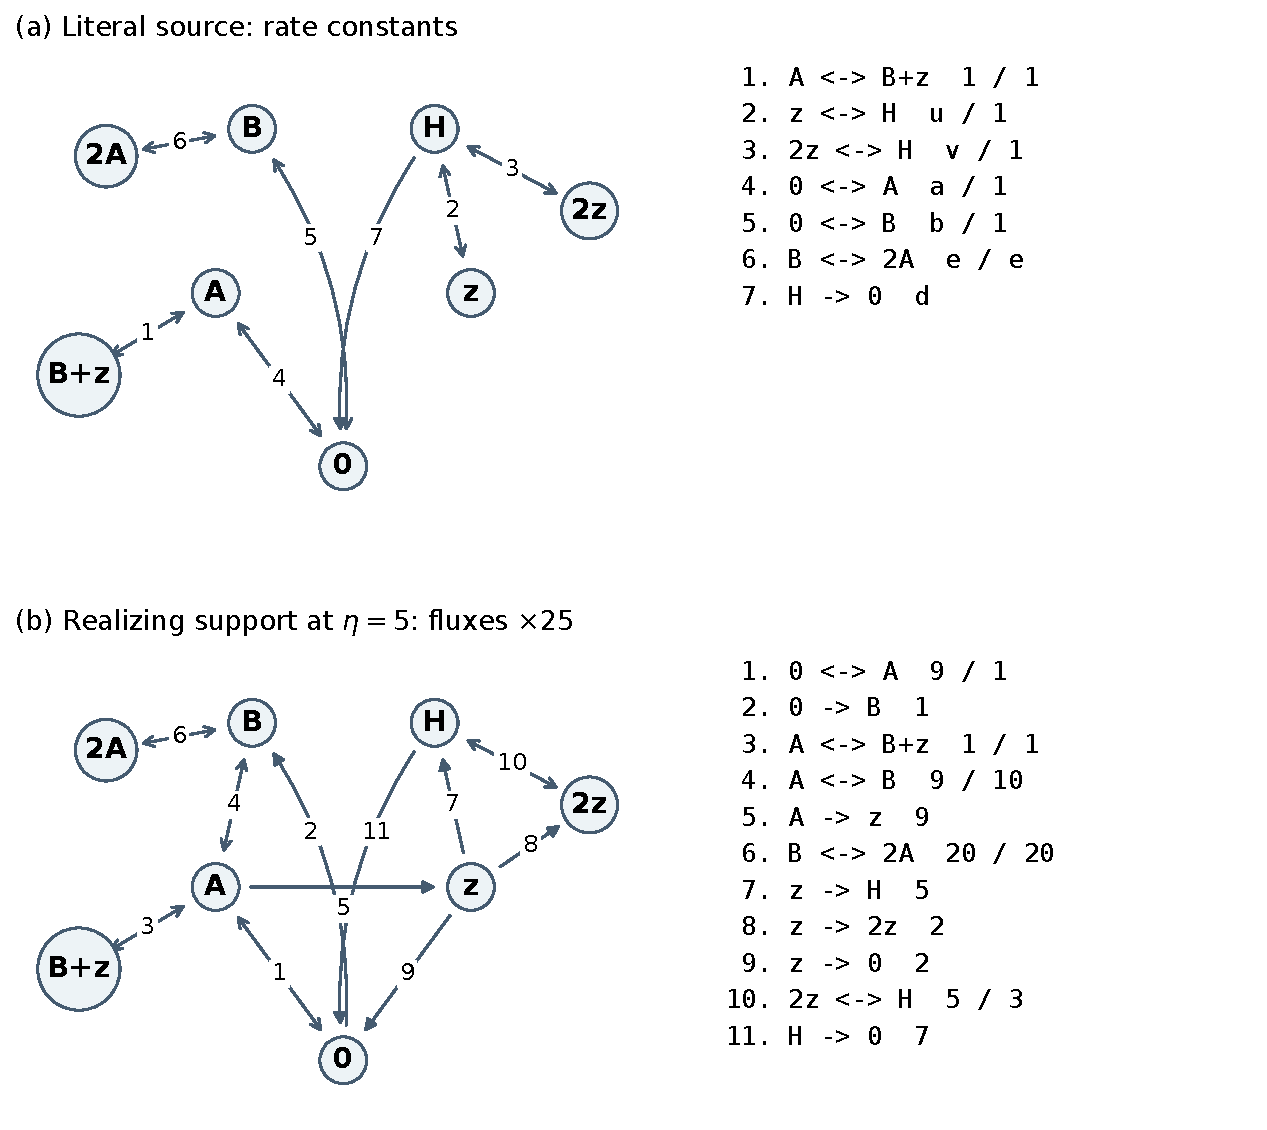
\includegraphics[width=\textwidth]{figures/networks.pdf}
\caption{(a) The literal source~\eqref{eq:source} with its rate constants. (b) The realizing support of Table~\ref{tab:flux} for the slice parameter $\eta=5$ of Section~\ref{sec:crossing}, labelled by $25$ times the fluxes; the edges $B\to0$, $A\to2A$ and $H\to z$ vanish there and are omitted. Numbered arrows refer to the keys on the right.}\label{fig:networks}
\end{figure}

\section{Scalar elimination: the parameter locus}\label{sec:locus}

\subsection{Monotonicity on the admissible half-line}

Write $\alpha=v(1+2d)/(2+d)>0$ and $\beta=u(1-d)/(2+d)$, so that $\rK(z)=\alpha z^2-\beta z$ and $z_0=\max\{0,\beta/\alpha\}$.

\begin{lemma}[Admissible domain and monotonicity]\label{lem:mono}
Let $p\in\Rp^6$.
\begin{enumerate}[label=(\roman*)]
\item For $z>0$, $\rK(z)\ge0$ if and only if $z\ge z_0$.
\item On $[z_0,\infty)$ the functions $\rK$ and $\rA$ are nonnegative and strictly increasing, $\rB$ is strictly decreasing, and $E$ is strictly increasing.
\item $E(0)=-\tfrac a2-\tfrac{ec}{2}<0$, and for $R=z_0+1+(1+e)c/b$ one has $E(R)>0$.
\end{enumerate}
\end{lemma}
\begin{proof}
(i) For $z>0$, $\rK(z)=z(\alpha z-\beta)\ge0$ if and only if $\alpha z\ge\beta$, which is $z\ge\beta/\alpha$; since $z>0$ this is $z\ge z_0$.

(ii) For $z_0\le x<y$,
\[
\rK(y)-\rK(x)=(y-x)\bigl(\alpha(x+y)-\beta\bigr)>0,
\]
because $\alpha x\ge\beta$ and $\alpha y>0$. Also $(z\rB(z))'=2c/(z+2)^2>0$, so $\rA=z\rB+\rK$ is strictly increasing, and $\rA\ge0$ on $[z_0,\infty)$ by (i). $\rB$ is strictly decreasing on $z>-2$. In $E=b-(1+e)\rB+\rK+e\rA^2$ the term $-(1+e)\rB$ is strictly increasing and $\rK$, $e\rA^2$ are nondecreasing (the latter because $\rA\ge0$ is nondecreasing), so $E$ is strictly increasing.

(iii) $\rB(0)=c/2$, $\rK(0)=\rA(0)=0$, so $E(0)=b-(1+e)c/2=-a/2-ec/2$. For $R$ as stated, $(1+e)\rB(R)=(1+e)c/(R+2)<(1+e)c\cdot b/((1+e)c)=b$ because $R+2>(1+e)c/b$; hence $E(R)>b-b+\rK(R)+e\rA(R)^2\ge0$, using $R\ge z_0$.
\end{proof}

\begin{lemma}[Admissible root]\label{lem:root}
$E$ has a root in $[z_0,\infty)$ if and only if $E(z_0)\le0$. The root is then unique, and it is positive.
\end{lemma}
\begin{proof}
If $E(z_*)=0$ with $z_*\ge z_0$ then $E(z_0)\le E(z_*)=0$ by monotonicity. Conversely, if $E(z_0)\le0$, then $E$ is continuous on $[z_0,R]$ (the only denominators are $z+2$ and $2+d$) and $E(R)>0$, so the intermediate value theorem gives a root; it is unique by strict monotonicity, and it is not $0$ because $E(0)<0$.
\end{proof}

\subsection{The threshold comparison}

\begin{lemma}[Root factorization]\label{lem:factor}
Let $z\ge z_0$ with $E(z)=0$. Then
\begin{equation}\label{eq:rootfactor}
(\rA(z)-s)\bigl[1+e(\rA(z)+s)\bigr]=(e-1)\rB(z)-es^2 ,
\end{equation}
and the bracket is positive. Consequently $\rA(z)\le s$ if and only if $t\le z$.
\end{lemma}
\begin{proof}
Expanding the left side gives $\rA-s+e\rA^2-es^2$, and by~\eqref{eq:port} with $E(z)=0$, $\rA-s+e\rA^2=(e-1)\rB$. The bracket is positive since $\rA(z)\ge0$ and $s>0$. Hence $\rA(z)\le s$ if and only if $(e-1)\rB(z)\le es^2$, that is, $(e-1)c\le es^2(z+2)$, which after division by $es^2>0$ is $z+2\ge c(e-1)/(es^2)$, i.e.\ $z\ge t$.
\end{proof}

\begin{lemma}[Residual at the threshold]\label{lem:threshold}
If $t\ge z_0$, then $(e-1)\rB(t)=es^2$ and
\begin{equation}\label{eq:Et}
E(t)=(\rA(t)-s)\bigl[1+e(\rA(t)+s)\bigr],
\end{equation}
so $E(t)\le0$ if and only if $\rA(t)\le s$. If $e\le1$, then $t\le-2<0\le z_0$.
\end{lemma}
\begin{proof}
From~\eqref{eq:cuts}, $t+2=c(e-1)/(es^2)$, so $\rB(t)=c/(t+2)=es^2/(e-1)$ (note $e>1$ when $t\ge z_0\ge0$). Substituting $(1-e)\rB(t)=-es^2$ into~\eqref{eq:port} gives $E(t)=\rA(t)-s+e\rA(t)^2-es^2$, which factors as stated. The bracket is positive as $\rA(t)\ge0$. If $e\le1$, the fraction in $t$ is nonpositive.
\end{proof}

\subsection{Proof of Theorem~\ref{thm:B}}

\begin{theorem}[Parameter locus]\label{thm:locus}
$p\in\DT$ if and only if $E(z_0)\le0$ and at least one of $e\le1$, $t\le z_0$, or $t>z_0$ and $\rA(t)\le s$ holds. On $\DT$ the balancing state is the lift $\ell(z_*)$ of the unique root $z_*\ge z_0$ of $E$.
\end{theorem}
\begin{proof}
Suppose $p\in\DT$, realized at a positive state $x$. By Theorem~\ref{thm:state}, $x$ is stationary with $K\ge0$ and $J\le B$. By Section~\ref{sec:prelim}, $x=\ell(z)$ with $z=x_z>0$ and $E(z)=0$; $K=\rK(z)\ge0$ gives $z\ge z_0$ by Lemma~\ref{lem:mono}(i), so $E(z_0)\le0$ by Lemma~\ref{lem:root}. By~\eqref{eq:reservoir}, $J\le B$ is $\rA(z)\le s$, hence $t\le z$ by Lemma~\ref{lem:factor}. If $e\le1$ or $t\le z_0$ we are done. Otherwise $t>z_0$ and $t\le z$ give $E(t)\le E(z)=0$ by monotonicity, hence $\rA(t)\le s$ by Lemma~\ref{lem:threshold}.

Conversely, suppose the criterion holds. Lemma~\ref{lem:root} gives the unique root $z_*\ge z_0$, $z_*>0$. We claim $t\le z_*$: if $e\le1$ then $t<0\le z_0\le z_*$; if $t\le z_0$ the same; and if $t>z_0$ with $\rA(t)\le s$, then $E(t)\le0=E(z_*)$ by Lemma~\ref{lem:threshold}, so $t\le z_*$ by monotonicity (both points lie in $[z_0,\infty)$). Lemma~\ref{lem:factor} then gives $\rA(z_*)\le s$. The lift $x=\ell(z_*)$ is positive: $\rB>0$, $z_*>0$, $\rH(z_*)>0$, and $\rA(z_*)=z_*\rB(z_*)+\rK(z_*)>0$ because $\rK(z_*)\ge0$. It is stationary, $K=\rK(z_*)\ge0$, and $J\le B$ by~\eqref{eq:reservoir}. Theorem~\ref{thm:state} gives the realization.
\end{proof}

\begin{corollary}[Safe region]\label{cor:safe}
If $d\ge1$ and $e\le1$ then $p\in\DT$.
\end{corollary}
\begin{proof}
For $d\ge1$, $\beta\le0$ so $z_0=0$, and $E(0)<0$ by Lemma~\ref{lem:mono}(iii); the branch $e\le1$ applies.
\end{proof}

\begin{remark}[Shape of the locus]\label{rem:shape}
The criterion shows that $\DT$ is closed relative to $\Rp^6$ and has nonempty interior; Figure~\ref{fig:region} shows a two-dimensional slice in which both mechanisms of failure are visible: for small loss $d$ the admissible cut $z_0$ is large and $E(z_0)>0$, so no stationary state carries a nonnegative fork current; for large reverse-channel rate $e$ the stationary state exists but its reverse-channel current exceeds the reservoir budget, $J>B$. Theorem~\ref{thm:open} shows that the complement of $\DT$ also has nonempty interior. In the full thirteen-dimensional rate space of~\eqref{eq:source} the disguised-toric locus is a contractible manifold with boundary~\cite{Boros2026}; we make no claim about the topology of the tied section beyond what the criterion states.
\end{remark}

\begin{figure}[htbp]\centering
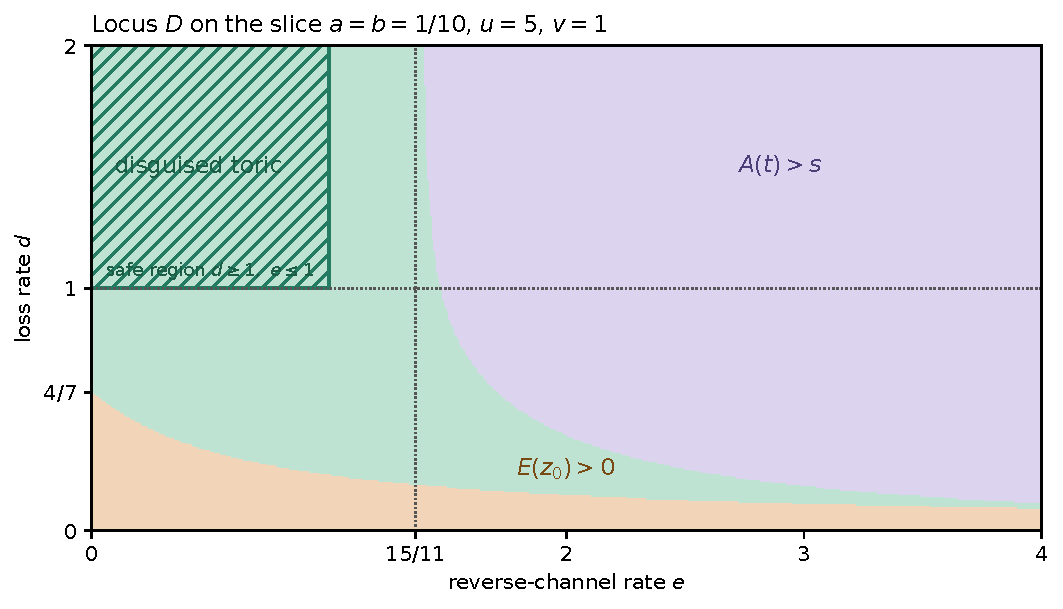
\includegraphics[width=.8\textwidth]{figures/region.pdf}
\caption{The locus $\DT$ on the slice $a=b=1/10$, $u=5$, $v=1$ in the $(e,d)$ plane, from the criterion of Theorem~\ref{thm:locus} evaluated on a grid. Green: disguised toric. Orange: $E(z_0)>0$, no admissible stationary state. Violet: an admissible stationary state exists but $\rA(t)>s$, i.e.\ $J>B$ there. The hatched box is the safe region of Corollary~\ref{cor:safe}. On this slice $t$ becomes positive at $e=15/11$, and for $e\to0$ the curve $E(z_0)=0$ meets the axis at $d=4/7$.}\label{fig:region}
\end{figure}

\subsection{Exact examples and productivity}\label{sec:examples}

The two cores of~\eqref{eq:source} have the oriented stoichiometry $\bigl(\begin{smallmatrix}-1&2\\1&-1\end{smallmatrix}\bigr)$, and a core is \emph{strictly productive} at a state if the net production vector of its two members is strictly positive~\cite{FeedbackBistability2026}. In terms of the source currents, the $AB$ core has production vector $(-K+2J,\,K-J)$, and the $zH$ core, oriented as $z\to H\to2z$, has $\bigl(-(uz-H)+2(H-vz^2),\ (uz-H)-(H-vz^2)\bigr)$, which at a stationary state equals $(-K,\,dH)$ by $\dot z=\dot H=0$.

\begin{proposition}\label{prop:productivity}
At any state realized as in Theorem~\ref{thm:state}, the $zH$ core is not strictly productive, since its first component is $-K\le0$. The $AB$ core can be strictly productive on $\DT$: for
\[
p=\bigl(\tfrac7{16},\tfrac7{16},1,\tfrac{12}{25},\tfrac12,1\bigr),\qquad x=\bigl(\tfrac12,\tfrac12,\tfrac58,\tfrac{13}{48}\bigr),
\]
the state is stationary with $K=\tfrac3{16}$ and $B-J=\tfrac38$, so $p\in\DT$, and both $AB$ margins equal $\tfrac1{16}$.
\end{proposition}
\begin{proof}
Direct substitution; the identities are exact rational arithmetic and are kernel-checked (Appendix~\ref{app:formal}).
\end{proof}

\begin{example}[An exact nontoric parameter with a unique stable equilibrium]\label{ex:negative}
Let
\[
p=\bigl(\tfrac{41729}{400000},\tfrac{115951}{800000},\tfrac1{100},5,5,10\bigr),\qquad
x=\bigl(\tfrac{703}{2000},\tfrac{9}{50},\tfrac{19}{100},\tfrac{19}{1250}\bigr).
\]
Then $x$ is stationary, $K=\tfrac{3173}{10000}>0$, but $2(B-J)=-\tfrac{81791}{400000}<0$. Since $d=10\ge1$, $z_0=0$ and $E$ is strictly increasing on $z\ge0$ by Lemma~\ref{lem:mono}, so the positive equilibrium is unique (as in~\cite{FeedbackBistability2026}) and no positive state satisfies Theorem~\ref{thm:state} and $p\notin\DT$. In the criterion, $z_0=0$, $E(0)<0$, $t>0$ and $\rA(t)>s$. The Jacobian at $x$ has characteristic polynomial
\[
\lambda^4+\tfrac{3121}{100}\lambda^3+\tfrac{5903829}{20000}\lambda^2+\tfrac{1595249817}{2000000}\lambda+\tfrac{847119843}{2000000},
\]
with Hurwitz determinants $\Delta_2=\tfrac{4207650123}{500000}$ and $\Delta_3=\tfrac{6299678574983809341}{10^{12}}$, both positive, so the equilibrium is hyperbolic and locally asymptotically stable. Failure of complex-balanced realizability is therefore not a stability boundary; Section~\ref{sec:crossing} makes this precise on a one-parameter slice and Theorem~\ref{thm:gas} shows that on $\DT$ the equilibrium is even globally stable.
\end{example}

\section{Permanence and global stability on the locus}\label{sec:dynamics}

\begin{theorem}[Permanence]\label{thm:permanence}
For every $p\in\Rp^6$ and every $x(0)\in\Rp^4$, the system~\eqref{eq:ode} has a unique solution defined for all $t\ge0$, which remains in $\Rp^4$. There are constants $0<m<M$, depending only on $p$, such that every such solution eventually remains in $[m,M]^4$. The constants can be chosen uniformly on each compact subset of $\Rp^6$; the entry times depend on the initial state.
\end{theorem}
\begin{proof}
\emph{Positive invariance.} The field is polynomial, hence locally Lipschitz, and quasipositive: on the face $A=0$ one has $\dot A=a+Bz+2eB\ge0$, on $B=0$, $\dot B=b+A+eA^2\ge0$, on $z=0$, $\dot z=A+3H\ge0$, and on $H=0$, $\dot H=uz+vz^2\ge0$. So the closed orthant is forward invariant on the maximal interval of existence. Moreover, on any bounded segment of a nonnegative solution each coordinate satisfies $\dot x_k\ge-\lambda x_k$ with a constant $\lambda$ depending on the bound (for instance $\dot A\ge-(2+2eA)A$ and $\dot z\ge-(B+u+2vz)z$), so $x_k(t)\ge x_k(0)e^{-\lambda t}>0$: a positive solution cannot reach the boundary in finite time.

\emph{An absorbing bound.} Let $L=(e+\tfrac32)A+(2e+1)B+z+\tfrac32H$. Expanding along~\eqref{eq:ode},
\begin{equation}\label{eq:ldot}
\dot L=(e+\tfrac32)a+(2e+1)b-A-B-(e+\tfrac12)Bz-2eA^2+\tfrac u2z-\tfrac v2z^2-\tfrac{3d}2H ,
\end{equation}
and the square identity
\begin{equation}\label{eq:square}
\frac{(u+2)^2}{8v}-z-\Bigl(\frac u2z-\frac v2z^2\Bigr)=\frac{(2vz-u-2)^2}{8v}\ \ge\ 0
\end{equation}
shows $\tfrac u2z-\tfrac v2z^2\le\tfrac{(u+2)^2}{8v}-z$. Dropping the nonpositive terms $-(e+\frac12)Bz-2eA^2$ on the closed orthant,
\begin{gather*}
\dot L\le C-A-B-z-\tfrac{3d}2H\le C-\rho L,\\
C=(e+\tfrac32)a+(2e+1)b+\frac{(u+2)^2}{8v},\qquad
\rho=\min\Bigl\{\frac1{e+3/2},\frac1{2e+1},1,d\Bigr\},
\end{gather*}
because $\rho(e+\frac32)A\le A$, $\rho(2e+1)B\le B$, $\rho z\le z$ and $\frac32\rho H\le\frac{3d}2H$. Integrating on the maximal interval,
\begin{equation}\label{eq:bound}
L(t)\le L(0)e^{-\rho t}+\frac C\rho\bigl(1-e^{-\rho t}\bigr).
\end{equation}
All weights of $L$ are at least one, so every coordinate is bounded by the right side of~\eqref{eq:bound} on the maximal interval. A solution bounded on a bounded maximal interval could be continued, so the solution is global. Eventually $L<2C/\rho=:M$, so every coordinate eventually stays below $M$.

\emph{Lower bounds.} Once $0\le A,B,z\le M$, dropping nonnegative terms in~\eqref{eq:ode} gives
\begin{equation}\label{eq:lower}
\dot A\ge a-(2+2eM)A,\quad \dot B\ge b-(1+e+M)B,\quad \dot z\ge A-(M+u+2vM)z,\quad \dot H\ge uz-(2+d)H ,
\end{equation}
where for instance $\dot A-\bigl(a-(2+2eM)A\bigr)=Bz+2eB+2eA(M-A)\ge0$ and $\dot z-\bigl(A-(M+u+2vM)z\bigr)=(M-B)z+2vz(M-z)+3H\ge0$. If $\dot y\ge\gamma-\lambda y$ with $\gamma,\lambda>0$ on $t\ge T$, then $y(t)\ge y(T)e^{-\lambda(t-T)}+(\gamma/\lambda)(1-e^{-\lambda(t-T)})$, so $y$ eventually exceeds $\gamma/(2\lambda)$. Applying this first to $A$ and $B$, then to $z$ with $A\ge m_A$, then to $H$ with $z\ge m_z$, gives eventual lower bounds
\[
m_A=\frac a{2(2+2eM)},\quad m_B=\frac b{2(1+e+M)},\quad m_z=\frac{m_A}{2(M+u+2vM)},\quad m_H=\frac{um_z}{2(2+d)},
\]
and $m=\min\{m_A,m_B,m_z,m_H\}$, decreased if necessary so that $m<M$.

\emph{Uniformity.} On a compact subset of $\Rp^6$ the quantity $C/\rho$ is bounded, so a common $M$ works; the bounds~\eqref{eq:lower} remain valid with the minima of $a,b,u$ and the maxima of $e,u,v,d$ over the set, which gives a common $m$. Only the entry time in~\eqref{eq:bound} depends on $L(0)$.
\end{proof}

\begin{lemma}[Full rank]\label{lem:rank}
Every realization of $f_p$ has stoichiometric subspace $\R^4$.
\end{lemma}
\begin{proof}
By~\eqref{eq:drift}, each coefficient vector $\cc_i$ lies in the span of the reaction vectors leaving the complex $y_i$ in the realization. The rows $0$, $B+z$, $z$ and $2z$ of~\eqref{eq:rows} have
\[
\det\begin{pmatrix}a&b&0&0\\1&-1&-1&0\\0&0&-u&u\\0&0&-2v&v\end{pmatrix}=-(a+b)uv\ne0 ,
\]
so the reaction vectors already span $\R^4$. This holds for every realization, in particular for the network of Table~\ref{tab:flux} on the boundaries where some of its edges vanish.
\end{proof}

\begin{theorem}[Global asymptotic stability on $\DT$]\label{thm:gas}
For every $p\in\DT$ the balancing state $\xs$ of Theorem~\ref{thm:locus} is the unique positive equilibrium of~\eqref{eq:ode}, and every solution with positive initial state converges to $\xs$; moreover $\xs$ is Lyapunov stable relative to $\Rp^4$.
\end{theorem}
\begin{proof}
Let $q$ be the balanced flux of Table~\ref{tab:flux} at $\xs$ and $k_{ij}=q_{ij}/(\xs)^{y_i}$ the rate constants. Consider the Horn--Jackson function~\cite{HornJackson1972}
\[
G(x)=\sum_{k=1}^4\Bigl[x_k\log\frac{x_k}{x_k^*}-x_k+x_k^*\Bigr],\qquad x\in\Rp^4,
\]
which is nonnegative, vanishes exactly at $\xs$, is strictly convex, and tends to infinity at the boundary of any compact subset of the closed orthant containing $\xs$ in its interior and at infinity. Along solutions, $\nabla G(x)=\log(x/\xs)$ and, by the full field equality of Theorem~\ref{thm:state}, with $\psi_i=(x/\xs)^{y_i}$,
\begin{equation}\label{eq:entropy}
\dot G=\sum_{i,j}k_{ij}x^{y_i}(y_j-y_i)\cdot\log\frac x{\xs}
=\sum_{i,j}q_{ij}\,\psi_i\log\frac{\psi_j}{\psi_i}
\ \le\ \sum_{i,j}q_{ij}(\psi_j-\psi_i)=0 ,
\end{equation}
using $r\log(s/r)\le s-r$ for $r,s>0$, with equality only if $r=s$, and Lemma~\ref{lem:circulation} with the potentials $\psi$. Equality in~\eqref{eq:entropy} forces $\psi_i=\psi_j$ on every edge with $q_{ij}>0$, i.e.\ $(y_j-y_i)\cdot\log(x/\xs)=0$ for every reaction of the realization; by Lemma~\ref{lem:rank} these vectors span $\R^4$, so $x=\xs$. Thus $\dot G<0$ on $\Rp^4\setminus\{\xs\}$. In particular no other positive equilibrium exists.

By Theorem~\ref{thm:permanence} every positive solution eventually lies in the compact set $[m,M]^4\subset\Rp^4$, on which $G$ is continuous. Along the solution $G$ is nonincreasing, hence converges to a limit $G_\infty$. The omega-limit set $\Omega$ is nonempty, compact, invariant and contained in $[m,M]^4$, and $G\equiv G_\infty$ on $\Omega$ by continuity. For a solution starting in $\Omega$, $G$ is constant, so $\dot G=0$ along it and the solution is identically $\xs$; hence $\Omega=\{\xs\}$ and the solution converges to $\xs$. Lyapunov stability follows from the sublevel sets of $G$: for any neighbourhood $N$ of $\xs$ there is $\varepsilon>0$ with $\{G<\varepsilon\}\subset N$, and this set is forward invariant because $G$ is nonincreasing.
\end{proof}

\begin{remark}
No general persistence result for weakly reversible or complex-balanced systems~\cite{Sontag2001,Anderson2011,GopalkrishnanMillerShiu2014,Craciun2015} is invoked: the literal feeds $0\to A$, $0\to B$ and the production chain provide the boundary control directly, and the same bounds hold off the locus. The convex functions $F_K,F_J$ of Section~\ref{sec:dual} live on exponent space and are unrelated to the entropy $G$ on concentration space. For $p$ in the safe region the realizing network is a single strongly connected linkage class of full rank, so global attraction could also be obtained from Anderson's single-linkage-class theorem~\cite{Anderson2011}; Theorem~\ref{thm:gas} covers the whole locus, including the boundaries where the realizing support loses edges.
\end{remark}

\section{A stable, productive crossing of the realizability boundary}\label{sec:crossing}

\begin{proposition}\label{prop:slice}
Consider the slice
\begin{equation}\label{eq:slice}
p_\eta=\Bigl(\frac{19-2\eta}{25},\ \frac{\eta-4}{25},\ 1,\ 5,\ \eta,\ 3\Bigr),\qquad 4<\eta<\frac{19}2,\qquad
\xs=\Bigl(\frac25,\frac15,\frac15,\frac2{25}\Bigr).
\end{equation}
For every $\eta$ in this interval, all six rate constants are positive, $\xs$ is the unique positive equilibrium of~\eqref{eq:ode}, it is hyperbolic and locally asymptotically stable, the system is disguised toric exactly when $\eta\le5$, and its $AB$ core is strictly productive at $\xs$ exactly when $\tfrac92<\eta<9$.
\end{proposition}
\begin{proof}
Positivity of $a=(19-2\eta)/25$ and $b=(\eta-4)/25$ is the stated interval. Substitution in~\eqref{eq:ode} gives $f_{p_\eta}(\xs)=0$ for every $\eta$, together with
\[
K=\frac9{25},\qquad B-A^2=\frac1{25},\qquad J=\frac\eta{25},\qquad
(-K+2J,\,K-J)=\Bigl(\frac{2\eta-9}{25},\ \frac{9-\eta}{25}\Bigr).
\]
Since $d=3\ge1$, $z_0=0$ and $E$ is strictly increasing on $z\ge0$, so every positive equilibrium is the lift of the unique root of $E$, and $\xs$ is the only one. Theorem~\ref{thm:state} at this unique equilibrium gives $p_\eta\in\DT$ if and only if $J\le B$, i.e.\ $\eta\le5$; the productivity interval is read off from the production vector.

The Jacobian of $f_{p_\eta}$ at $\xs$ is
\begin{equation}\label{eq:jac}
Df_{p_\eta}(\xs)=\begin{pmatrix}
-2-\tfrac{8\eta}5&\tfrac15+2\eta&\tfrac15&0\\[2pt]
1+\tfrac{4\eta}5&-\tfrac65-\eta&-\tfrac15&0\\[2pt]
1&-\tfrac15&-\tfrac{26}5&3\\[2pt]
0&0&3&-5
\end{pmatrix},
\end{equation}
with characteristic polynomial $\lambda^4+c_1\lambda^3+c_2\lambda^2+c_3\lambda+c_4$,
\begin{equation}\label{eq:char}
c_1=\frac{67+13\eta}5,\quad c_2=\frac{1290+707\eta}{25},\quad c_3=\frac{1885+1558\eta}{25},\quad c_4=\frac{905+769\eta}{25}.
\end{equation}
The Hurwitz determinants are
\begin{align*}
\Delta_2&=c_1c_2-c_3=\frac{77005+56349\eta+9191\eta^2}{125},\\
\Delta_3&=c_1c_2c_3-c_3^2-c_1^2c_4\\
&=\frac{124841700+201048900\,\eta+97654062\,\eta^2+13669773\,\eta^3}{3125}.
\end{align*}
All coefficients of $c_1,\dots,c_4,\Delta_2,\Delta_3$ as polynomials in $\eta$ are positive, so these quantities are positive for every $\eta>0$. By the Routh--Hurwitz criterion for a quartic~\cite{Gantmacher1959} (positivity of $c_1$, $\Delta_2$, $\Delta_3$ and $c_4\Delta_3$), every eigenvalue has negative real part; the linearization theorem gives hyperbolicity and local asymptotic stability. In particular nothing happens to the spectrum at $\eta=5$.
\end{proof}

\begin{figure}[htbp]\centering
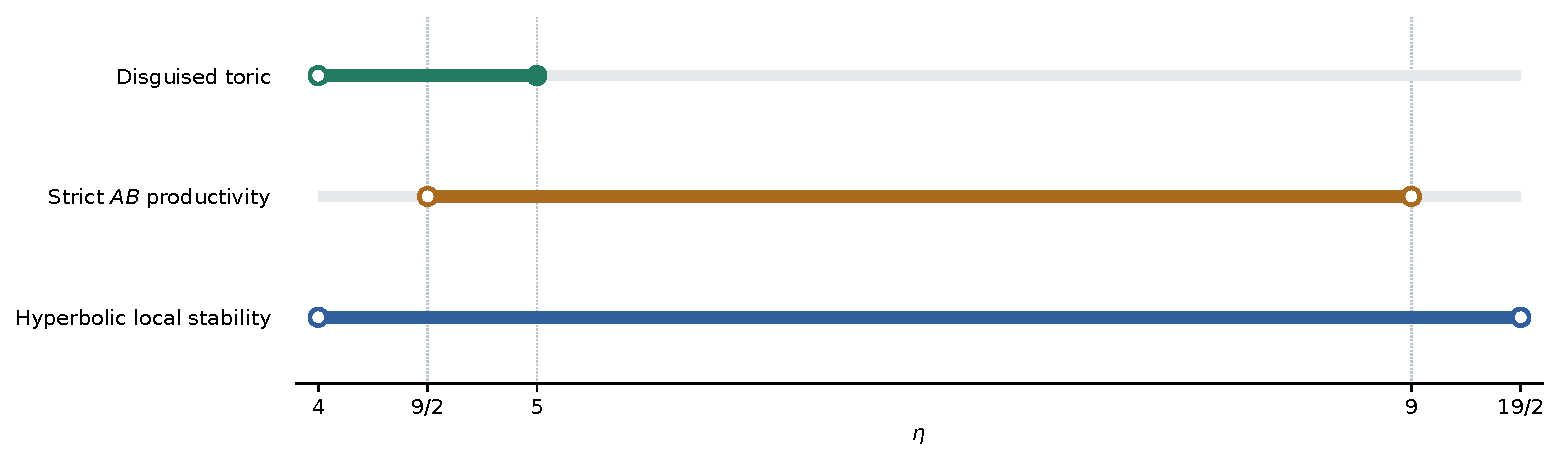
\includegraphics[width=\textwidth]{figures/intervals.pdf}
\caption{Exact classification of the slice~\eqref{eq:slice}. Filled endpoints are included, hollow endpoints excluded. Local hyperbolic stability holds on the whole interval; global stability holds on the toric part $\eta\le5$ by Theorem~\ref{thm:gas} and on a neighbourhood extending past $5$ by Theorem~\ref{thm:open}.}\label{fig:intervals}
\end{figure}

\begin{theorem}[An open, productive, globally attracting nontoric region]\label{thm:open}
There is a nonempty open set $\mathcal U\subset\Rp^6\setminus\DT$ such that for every $p\in\mathcal U$ the system~\eqref{eq:ode} has a unique positive equilibrium, this equilibrium is globally asymptotically stable relative to $\Rp^4$, and its $AB$ core is strictly productive.
\end{theorem}
\begin{proof}
Let $p_0=p_5=(\tfrac9{25},\tfrac1{25},1,5,5,3)\in\DT$ with balancing state $\xs$. Since $Df_{p_0}(\xs)$ is nonsingular, the implicit function theorem gives a neighbourhood $P_1$ of $p_0$ and a smooth map $p\mapsto x_p$ with $x_{p_0}=\xs$ and $f_p(x_p)=0$. Shrink $P_1$ to have compact closure in $\Rp^6$ and $d>1$ on it; then $z_0=0$ and the elimination of Section~\ref{sec:locus} shows that $x_p$ is the unique positive equilibrium of $f_p$ for $p\in P_1$. By the uniform part of Theorem~\ref{thm:permanence} there is a compact box $Q=[m,M]^4$ into which every positive solution of every system $p\in\overline{P_1}$ eventually enters and remains; enlarging $Q$ slightly we may assume that all $x_p$, $p\in P_1$, lie in the interior of $Q$.

Let $V_p(x)=G(x\mid x_p)$ be the Horn--Jackson function centred at $x_p$ and $W(p,x)=\nabla V_p(x)\cdot f_p(x)=\log(x/x_p)\cdot f_p(x)$, a smooth function on $P_1\times\Rp^4$. At $p_0$ the proof of Theorem~\ref{thm:gas} gives $W(p_0,x)<0$ for $x\ne\xs$. We need a uniform version near the moving zero. First, $W(p,x_p)=0$ and $\nabla_xW(p,x_p)=0$ for all $p\in P_1$, because $f_p(x_p)=0$ and $\nabla V_p(x_p)=0$. Second, the Hessian of $W(p_0,\cdot)$ at $\xs$ is negative definite. Intrinsically, write $x=\xs e^{w}$ coordinatewise; then $\psi_i=e^{y_i\cdot w}$ and~\eqref{eq:entropy} expands as
\[
\dot G=\sum_{i,j}q_{ij}e^{y_i\cdot w}(y_j-y_i)\cdot w
=\sum_{i,j}q_{ij}(y_j-y_i)\cdot w+\sum_{i,j}q_{ij}(y_i\cdot w)\bigl((y_j-y_i)\cdot w\bigr)+O(|w|^3),
\]
where the first sum vanishes since $\sum_{i,j}q_{ij}(y_j-y_i)=f_{p_0}(\xs)=0$, and the second equals $-\tfrac12\sum_{i,j}q_{ij}\bigl((y_j-y_i)\cdot w\bigr)^2$ by vertex balance (Lemma~\ref{lem:circulation} with the potentials $(y_i\cdot w)^2$). This quadratic form is negative definite by Lemma~\ref{lem:rank}. Concretely, with $D=\diag(1/x_k^*)$ the Hessian is $-2Q_0$ with
\[
Q_0=-\tfrac12\bigl[D\,Df_{p_0}(\xs)+Df_{p_0}(\xs)^{\mathsf T}D\bigr],
\]
whose leading principal minors, computed exactly from~\eqref{eq:jac} at $\eta=5$, are
\begin{equation}\label{eq:minors}
25,\qquad \frac{2199}{16},\qquad \frac{55245}{16},\qquad \frac{31001025}{256},
\end{equation}
all positive. By continuity of the second derivatives of $W$ in $(p,x)$, there are $r>0$, $\gamma>0$ and a smaller neighbourhood $P_2\subset P_1$ of $p_0$ such that the Hessian of $W(p,\cdot)$ is at most $-2\gamma$ on the ball of radius $r$ about $x_p$ for all $p\in P_2$; Taylor's theorem with the two vanishing conditions then gives
\[
W(p,x)\le-\gamma\,\|x-x_p\|^2\qquad\text{for }\|x-x_p\|\le r,\ p\in P_2 .
\]
On the compact set $Q\setminus B(\xs,r/2)$ the continuous function $W(p_0,\cdot)$ has a strictly negative maximum, and by uniform continuity of $W$ on $\overline{P_2}\times Q$ there is a neighbourhood $P_3\subset P_2$ on which $W(p,\cdot)<0$ on $Q\setminus B(\xs,r/2)$ and $\|x_p-\xs\|<r/2$. The two estimates cover $Q$: for $p\in P_3$, $W(p,x)<0$ for all $x\in Q\setminus\{x_p\}$.

Every positive solution of a system $p\in P_3$ eventually stays in $Q$, where $V_p$ is a strict Lyapunov function; the omega-limit argument of Theorem~\ref{thm:gas} gives convergence to $x_p$, and the sublevel sets of $V_p$ inside $Q$ give Lyapunov stability. (Nearby nontoric systems need not retain any complex-balanced realization; only the Lyapunov decrease is transferred, not the realization.)

At $p_0$ the $AB$ margins are $-K+2J=\tfrac1{25}$ and $K-J=\tfrac4{25}$, positive; they depend continuously on $p$ along the branch. Choose $\eta>5$ so close to $5$ that $p_\eta\in P_3$. At its unique equilibrium $\xs$, $J-B=(\eta-5)/25>0$, and by continuity of the branch this strict inequality, the strict margins and the inclusion in $P_3$ persist on an open neighbourhood $\mathcal U$ of $p_\eta$ in $\Rp^6$. For $p\in\mathcal U$ the unique positive equilibrium violates $J\le B$, so by Theorem~\ref{thm:state} no complex-balanced realization exists and $\mathcal U\cap\DT=\varnothing$.
\end{proof}

\begin{remark}
Global stability of perturbations of complex-balanced systems is studied in general by Yu~\cite{Yu2022} under a robust permanence hypothesis; here the estimates are verified directly on the common absorbing box supplied by Theorem~\ref{thm:permanence}, and no explicit perturbation radius is claimed. The example shows that the boundary of the disguised-toric locus need not be a bifurcation set and need not separate productive from unproductive operation of an autocatalytic core.
\end{remark}

\section{Finite catalytic attachments}\label{sec:assembly}

Fix $m\ge0$, private species $W_1,\dots,W_m$, catalyst complexes $Y_r\in\N^4$ in the base species (arbitrary nonnegative integer multiplicities, possibly coinciding with source complexes of~\eqref{eq:source} or with each other), and rate constants $\alpha_r,\beta_r>0$. Adjoin the reversible reactions
\begin{equation}\label{eq:attach}
Y_r\ \rev{\alpha_r}{\beta_r}\ Y_r+W_r,\qquad 1\le r\le m .
\end{equation}
Coincident complexes are merged and parallel rate constants added. The enlarged mass-action field on $\R^{4+m}$ is triangular:
\begin{equation}\label{eq:triangular}
\dot x=f_p(x),\qquad \dot W_r=x^{Y_r}(\alpha_r-\beta_rW_r).
\end{equation}
Competing realizations may now use any finite set of complexes in $\N^{4+m}$, including complexes mixing base and private species.

\begin{theorem}[Catalytic attachment closure]\label{thm:assembly}
For every finite choice in~\eqref{eq:attach}, the enlarged system~\eqref{eq:triangular} is disguised toric if and only if $p\in\DT$. When $p\in\DT$, adjoining~\eqref{eq:attach} to the realization of Table~\ref{tab:flux} gives a realization complex balanced at $(\xs,W^*)$ with $W_r^*=\alpha_r/\beta_r$. Every positive solution of~\eqref{eq:triangular} is global and permanent, the enlarged system has a positive equilibrium exactly above each positive equilibrium of the base system, and whenever a base equilibrium is globally asymptotically stable relative to $\Rp^4$, the equilibrium $(x_p,W^*)$ above it is globally asymptotically stable relative to $\Rp^{4+m}$. This applies on $\DT$ and on the open set of Theorem~\ref{thm:open}.
\end{theorem}
\begin{proof}
\emph{Sufficiency.} Let $p\in\DT$ and embed the base realization with private exponents zero. Each pair~\eqref{eq:attach} is detailed balanced at $(\xs,W^*)$ because $\alpha_r(\xs)^{Y_r}=\beta_r(\xs)^{Y_r}W_r^*$, and its net contribution to the field is exactly the second line of~\eqref{eq:triangular}. Balanced contributions add at coinciding vertices, so the union is complex balanced at $(\xs,W^*)$ and realizes~\eqref{eq:triangular}.

\emph{Necessity.} Suppose some realization of~\eqref{eq:triangular} is complex balanced at a positive $(x,W)$. Summing its drift equations, as in Corollary~\ref{cor:necessity}, shows that $(x,W)$ is stationary, so $f_p(x)=0$. Now fix one of the two certificates $(h,\pi)$ of Table~\ref{tab:dual} and apply Lemmas~\ref{lem:dual} and~\ref{lem:extend} to the \emph{projected} data: to every vertex $\tilde y\in\N^{4+m}$ of the realization assign the base exponent $\pi_{\text{base}}(\tilde y)\in\N^4$, to the eight vertices $(y_i,0)$ the prescribed data $(h_i,\pi_i)$, and to every other vertex an active piece of $F$ at $\pi_{\text{base}}(\tilde y)$ with the corresponding slope and potential. The supporting inequalities~\eqref{eq:support} hold for the projected exponents by Lemma~\ref{lem:extend} (with the projections of auxiliary vertices as the additional points, which may coincide with base source complexes; they are treated as separate vertices with their own active piece). The base coordinates of the drift equations of the realization are vertex-balanced flux equations with drifts equal to the base parts of the coefficient rows of~\eqref{eq:triangular}, and those base parts are $x^{y_i}\cc_i$ at $(y_i,0)$ and zero at every other vertex, because the base field $f_p(x)$ contains no private species and the attachment monomials only affect the private coordinates. Lemma~\ref{lem:dual} in the base coordinates therefore yields $\sum_ih_i\cdot x^{y_i}\cc_i\ge0$, that is $K\ge0$ and, using stationarity of $x$, $J\le B$. Theorem~\ref{thm:state} gives $p\in\DT$.

\emph{Dynamics.} The base solution $x(t)$ is global and permanent by Theorem~\ref{thm:permanence} and is unaffected by $W$. Each private coordinate solves a scalar linear equation with the explicit solution
\[
W_r(t)-W_r^*=\bigl(W_r(0)-W_r^*\bigr)\exp\Bigl[-\beta_r\int_0^tx(s)^{Y_r}\,ds\Bigr],
\]
so $W_r(t)$ stays between $W_r(0)$ and $W_r^*$: it is positive and bounded, hence global. Permanence of $x$ gives an eventual positive lower bound on $x^{Y_r}$, so the integral diverges and $W_r(t)\to W_r^*$; in particular $W_r$ eventually lies in $[W_r^*/2,2W_r^*]$, which with the base bounds proves permanence. At a positive stationary point $\dot W_r=0$ forces $W_r=W_r^*$, so equilibria of~\eqref{eq:triangular} are exactly the points $(x_p,W^*)$ above base equilibria $x_p$. If $x(t)\to x_p$ then $(x,W)(t)\to(x_p,W^*)$. For Lyapunov stability, the private deviations $|W_r(t)-W_r^*|$ are nonincreasing in time and the base coordinates do not depend on $W$, so a neighbourhood of $(x_p,W^*)$ that is a product of a base neighbourhood supplied by base stability and a private box is forward invariant up to the chosen tolerance.
\end{proof}

\begin{remark}
The theorem quantifies over arbitrarily many attachments and over unrestricted competing realizations in the enlarged species space. Its decisive hypothesis is that the attachment reactions have zero base projection, so that they cannot offset a negative base certificate budget. A module whose drift has nonzero base projection, such as a second feedback loop through $A$ or $z$, can in principle change the classification, and the argument does not apply to it; see Section~\ref{sec:discussion}.
\end{remark}

\section{Discussion}\label{sec:discussion}

\paragraph{What was computed.} The disguised-toric locus of the tied family~\eqref{eq:source} is described exactly by two inequalities at the unique admissible root of a one-variable function. Membership is decided by a finite computation: evaluate $E$ at $z_0$, and if $e>1$ and $t>z_0$, evaluate $\rA$ at $t$. The two flux budgets $K\ge0$ and $J\le B$ have a direct reading: the fork $A\rightleftarrows B+z$ must not run backwards at the balancing state, and the reverse channel $B\rightleftarrows2A$ may run in either direction but its forward current is capped by the reservoir exchange of $B$. The convex functions $F_K$ and $F_J$ are the exact obstructions certifying that no auxiliary complexes, of any molecularity, can circumvent either constraint.

\paragraph{Relation to general theory.} Flux-based and algebraic descriptions of the disguised-toric locus~\cite{Boros2026,MullerDeshpandeRegensburger2026} treat the full rate space of a network. Here the six parameters trace a section of that space, and the certificate method exploits the tied structure: because the source complexes are fixed and few, two certificates with all $64$ supporting inequalities verified once suffice for every parameter and state. General results about the full locus, such as contractibility, do not automatically transfer to a section, and none is used. Conversely, the section exhibits phenomena that the general theory only predicts abstractly: an explicit boundary of the locus where the realizing support loses edges but the equilibrium remains globally stable, and an explicit open nontoric region with the same qualitative dynamics.

\paragraph{Consequences for the autocatalytic assembly.} On $\DT$ the assembly has a single, globally attracting positive state, so the bistability found in the companion manuscript for small $e$~\cite{FeedbackBistability2026} necessarily occurs outside $\DT$; the criterion locates a large explicit region in which such behaviour is excluded for all initial conditions, with an explicit Lyapunov function. At the same time, complex balance forbids strict productivity of the $zH$ core at equilibrium, while the $AB$ core can be productive on and off the locus. The realizability boundary is therefore neither a stability boundary nor an activity boundary. Deterministic vector-field equality also does not identify stochastic jump processes, so no product-form stationary distribution of the original network is implied by a realizing graph.

\paragraph{Open questions.} The composition problem is to describe how the certificate budgets change when two modules are joined through shared species with nonzero projected drift; Theorem~\ref{thm:assembly} settles the case of zero projection. A universal composition law for feedback-coupled assemblies, and an intrinsic description of the boundary of the tied section, remain open.

\appendix
\section{Formal verification and reproduction}\label{app:formal}

\subsection{Scope of the Lean development}

The classification results are formalized in Lean~4 (toolchain \texttt{v4.30.0}) with Mathlib~\cite{Lean4,Mathlib} in the modules listed in Table~\ref{tab:modules}; the source system is imported from the companion development, not restated. The formal definition of realizability at a state is
\begin{verbatim}
def ExtendedCertificate {n : Nat} (p : Rates) (x : State)
    (z : Fin n -> Fin 4 -> Nat)
    (q : Sum (Fin 8) (Fin n) -> Sum (Fin 8) (Fin n) -> Real) :
    Prop :=
  (forall i j, 0 <= q i j) and (forall i, q i i = 0) and
  (forall i, sum j, q i j = sum j, q j i) and
  (forall i k, sum j, q i j *
      (extendedComplexes z j k - extendedComplexes z i k)
    = extendedRows p x i k)

def RealizableAt (p : Rates) (x : State) : Prop :=
  exists n, exists z : Fin n -> Fin 4 -> Nat,
    exists q : Sum (Fin 8) (Fin n) -> Sum (Fin 8) (Fin n) -> Real,
      ExtendedCertificate p x z q

def DisguisedToric (p : Rates) : Prop :=
  exists x : State, x.Positive and RealizableAt p x
\end{verbatim}
Here \lean{extendedComplexes z} adjoins $n$ arbitrary complexes in $\N^4$ to the eight source complexes and \lean{extendedRows p x} is the coefficient row $x^{y_i}\cc_i$ at source complexes and zero at the adjoined ones. The two exported family theorems are
\begin{verbatim}
theorem cac_state_characterization (p : Rates) (x : State)
    (hp : p.Positive) (hx : x.Positive) :
    RealizableAt p x <-> Stationary p x and 0 <= x.A - x.B*x.z
                         and p.e*(x.B - x.A^2) <= x.B

theorem cacParameterLocus (p : Rates) (hp : p.Positive) :
    DisguisedToric p <-> ParameterCriterion p
\end{verbatim}
with \lean{ParameterCriterion} the criterion of Theorem~\ref{thm:locus} written with the reduced functions of~\eqref{eq:reduced}. The thin endpoint \lean{cacFamilyResolution} conjoins the parameter criterion, the constructive witness \lean{criterion_literal_witness} (nonnegative rate constants indexed by the eight source complexes, zero diagonal, complex balance at the balancing state written with ordinary monomials, and the identity \lean{auxiliaryDerivative (realizingRates p x) y = sourceDerivative p y} for every state \lean{y}), the safe region, and the negative example with its uniqueness and nonrealizability.

\begin{table}[htbp]\centering\small
\caption{Lean modules under \texttt{proofs/DisguisedToricAssemblies/} and their contents.}\label{tab:modules}
\begin{tabular}{>{\raggedright\arraybackslash}p{.30\textwidth}>{\raggedright\arraybackslash}p{.62\textwidth}}\toprule
Module&Content\\\midrule
\lean{ConvexDual.lean}&Lemmas~\ref{lem:circulation}, \ref{lem:dual}, \ref{lem:extend} for arbitrary finite vertex types (\lean{circulation_potential}, \lean{supporting_dual_nonneg}, \lean{complete_supports}).\\
\lean{CACFluxConstruction.lean}&Coefficient rows~\eqref{eq:rows}, the flux table, its nonnegativity, balance and drift identities (\lean{coefficient_source}, \lean{flux_table_balanced}, \lean{flux_table_drift}, \lean{flux_nonneg}).\\
\lean{CACNecessary.lean}&The two certificates, all $2\times64$ slacks by exhaustive case analysis, and the pairings~\eqref{eq:pairings} (\lean{dual_support}, \lean{current_support}, \lean{dual_evaluation}, \lean{current_evaluation}).\\
\lean{CACSufficient.lean}, \lean{BalancedFlux.lean}&Proposition~\ref{prop:flux} and the rate reconstruction (\lean{cac_flux_certificate}, \lean{cac_constructive_sufficiency}).\\
\lean{ExtendedFlux.lean}&Unrestricted necessity and Theorem~\ref{thm:state} (\lean{extended_necessary}, \lean{cac_state_characterization}).\\
\lean{CACLocusAnalysis.lean}, \lean{CACRootExistence.lean}, \lean{CACThreshold.lean}&Lemmas~\ref{lem:mono}--\ref{lem:threshold} (\lean{K_nonneg_iff_cut}, \lean{admissible_increasing}, \lean{admissible_root_exists}, \lean{root_threshold_comparison}, \lean{threshold_residual_sign}).\\
\lean{CACParameterLocus.lean}&Theorem~\ref{thm:locus} (\lean{cacParameterLocus}).\\
\lean{LiteralRealization.lean}&Ordinary monomials and full field equality (\lean{activity_monomial}, \lean{realizing_field_eq}, \lean{criterion_literal_witness}).\\
\lean{CACExamples.lean}, \lean{Main.lean}&Proposition~\ref{prop:productivity}, Example~\ref{ex:negative} (stationarity, uniqueness, nonrealizability, the value $-81791/400000$), Corollary~\ref{cor:safe}, and the endpoint \lean{cacFamilyResolution}.\\
\lean{CACDissipativity.lean}&Identities~\eqref{eq:ldot}, \eqref{eq:square}, the bound $\dot L\le C-\rho L$ and the comparison inequalities~\eqref{eq:lower} as algebraic statements (\lean{massDrift_identity}, \lean{square_dissipation}, \lean{massDrift_coercive}, \lean{scalar_lower_bounds}).\\
\lean{CACStableSlice.lean}, \lean{Postproof.lean}&Slice positivity, stationarity, uniqueness, the toric threshold $\eta\le5$, the productivity interval, and positivity of $c_1,\dots,c_4,\Delta_2,\Delta_3$ for all $\eta>0$ (\lean{slice_toric_iff}, \lean{slice_productivity}, \lean{slice_hurwitz}).\\\bottomrule
\end{tabular}
\end{table}

\subsection{Division of evidence}

Table~\ref{tab:coverage} states, claim by claim, what is kernel-checked and what is conventional. The formal statements use natural exponents, strictly positive real rate constants and states, and arbitrary finite sets of additional complexes. The verification was run with warnings treated as errors and without \texttt{sorry}; the exported theorems depend only on the axioms \texttt{Classical.choice}, \texttt{Quot.sound} and \texttt{propext}. The receipts record the toolchain, the hash of the frozen Mathlib manifest, source hashes and the elaborated theorem statements; the family endpoint verified in $157$ seconds and the slice and dissipativity module in $113$ seconds.

\begin{table}[htbp]\centering\small
\caption{Kernel-checked and conventional parts of each result.}\label{tab:coverage}
\begin{tabular}{>{\raggedright\arraybackslash}p{.34\textwidth}>{\raggedright\arraybackslash}p{.58\textwidth}}\toprule
Result&Evidence\\\midrule
Theorem~\ref{thm:state} (state criterion, rate reconstruction, full field equality)&Lean, including arbitrary finite auxiliary complexes.\\
Theorem~\ref{thm:locus}, Corollary~\ref{cor:safe}&Lean.\\
Proposition~\ref{prop:productivity}, Example~\ref{ex:negative}&Lean for stationarity, the values of $K$ and $B-J$, uniqueness, nonrealizability and the margins; the characteristic polynomial and Hurwitz determinants of the example are exact rational computations reproduced by the check script, and the stability conclusion is conventional.\\
Theorem~\ref{thm:permanence}&Algebraic identities and comparison inequalities in Lean; positive invariance, continuation and the trajectory conclusions conventional.\\
Lemma~\ref{lem:rank}, Theorem~\ref{thm:gas}&Conventional; the determinant is reproduced by the check script.\\
Proposition~\ref{prop:slice}&Slice algebra and the positivity of all Hurwitz quantities in Lean; the characteristic polynomial is an exact symbolic computation reproduced by the check script; Routh--Hurwitz and linearization conventional.\\
Theorem~\ref{thm:open}, Theorem~\ref{thm:assembly}&Conventional; the minors~\eqref{eq:minors} are reproduced by the check script.\\\bottomrule
\end{tabular}
\end{table}

\subsection{Reproduction}

From the repository root, the strict verifier is invoked as
\begin{verbatim}
python scripts/verify_proof.py proofs/DisguisedToricAssemblies/Main.lean
    --timeout 300
    --declaration DisguisedToricAssemblies.cacFamilyResolution
    --declaration DisguisedToricAssemblies.cacParameterLocus
\end{verbatim}
and analogously for \lean{Postproof.lean} with the declarations \lean{slice_toric_iff}, \lean{slice_hurwitz} and \lean{massDrift_coercive}. The script \texttt{check\_paper.py} distributed with the sources re-derives, in exact rational and symbolic arithmetic, every number printed in this paper: the coefficient rows, all $128$ certificate slacks and both pairings, the closed forms of $F_K$ and $F_J$, the balance and drift identities of Table~\ref{tab:flux}, the reduced-function identities~\eqref{eq:combinations}, \eqref{eq:port}, \eqref{eq:rootfactor} and~\eqref{eq:Et}, the identities~\eqref{eq:ldot}, \eqref{eq:square} and~\eqref{eq:lower}, the determinant of Lemma~\ref{lem:rank}, both examples, the Jacobian~\eqref{eq:jac}, the coefficients~\eqref{eq:char}, the Hurwitz determinants, the minors~\eqref{eq:minors}, and the fluxes of Figure~\ref{fig:networks}(b). The figures are generated by \texttt{make\_figures.py}; the region plot evaluates the exact criterion on a grid and involves no sampling of realizations.

\bibliographystyle{plain}
\bibliography{refs}

\end{document}
